% select document class
\documentclass[11pt,a4paper]{article}

% include packages
\usepackage[T1]{fontenc}
\usepackage[ngerman]{babel}
\usepackage[autostyle=true]{csquotes}
\usepackage{amsmath}
\usepackage{amssymb}
\usepackage{mathtools}
\usepackage{siunitx}
\AtBeginDocument{\RenewCommandCopy\qty\SI}
\usepackage{physics}
\usepackage{graphicx}
\usepackage{hyperref}
\usepackage{geometry}
\usepackage{dsfont}
\usepackage{stmaryrd}

% setup for packages
\hypersetup{colorlinks=true, linkcolor=black, citecolor=black}
\geometry{
 a4paper,
 total={170mm,257mm},
 left=20mm,
 top=20mm,
 }
\graphicspath{{figs/}}

% generate title
\title{\textbf{Computerphysik SS 2023 \\ Hausaufgabe 5}}
\author{Gabriel Remiszewski und Christian Fischer}
\date{08. Juli 2023}

% document
\begin{document}

\maketitle

\section*{H.1: Frequenzabhängige Fehlerdämpfung mit Multigrid}\label{sec:h1}

In dieser Aufgabe wird das Randwertproblem
\begin{equation*}
    u''(x) = 0 , \quad u(0) = 0 = u(\pi) ,
\end{equation*} betrachtet. Werden die Randbedingungen für die allgemeine Lösung $u(x) = Ax + B$ ($A,B = \mathrm{const.}$) ausgewertet, so ergibt sich $u(x) = 0$ als spezielle (exakte) Lösung
des betrachteten Randwertproblems. Nun soll das in der Vorlesung vorgestellte Multigrid-Verfahren an diesem Problem getestet werden und numerisch die erwartete analytische Lösung liefern.\newline

\noindent 
1. Zunächst wird das Multigrid-Verfahren für den V-Zyklus ($\gamma = 1$) mit variabler Anzahl von Levels implementiert. Dabei geht der Multigrid-Zyklus von einer Näherungslösung $v_h$ für das Gleichungsystem $A_h u_h = f_h$ auf dem
feinsten Gitter $G_h$ mit Schrittweite $h$ aus. Es wird das Gauss-Seidel Verfahren als Glättoperator verwendet und für beide Aufgaben eine lineare Differentialgleichung
angenommen, weshalb die Matrix unter diesen Bedingungen folgende Form bekommt:
\[(A_h)_{ij} = \frac{1}{h^2}
\begin{cases}
2 - h^2g_i & i = j\\
-1 & i = j\pm 1\\
0 & \text{sonst}
\end{cases} \qquad i,j\in[1,N-1]\]
Hier wird der Algorithmus beispielhaft für zwei Levels vorgestellt. In einem ersten Schritt (Glättung) werden mit dem Gauß-Seidel-Verfahren $\nu_{\mathrm{pre}}$ Dämpfungsschritte durchgeführt, es wird also $w_h = \mathcal{G}(R)^{\nu_{\mathrm{pre}}} v_h$ (hierbei ist $R$ der Relaxationsparameter) berechnet.
In einem zweiten Schritt (Restriktion und Rekursion) wird der Residuenvektor $r_h = f_h - A_h w_h$ berechnet. 
Es müssen nun zwei Fälle unterschieden werden. Falls $h<h_{\mathrm{max}}$ (das gröbste Gitter ist noch nicht erreicht), wird aus dem Residuenvektor die neue rechte Seite für das gröbere
Gitter $f_{2h} = \mathcal{I}_h^{2h} r_h$ berechnet. Der Projektionsoperator $\mathcal{I}_h^{2h}$ bildet ein Feld $w_h$ von einem feineren auf das gröbere Gitter gemäß folgender Abbildungsvorschrift ab:
\begin{equation*}
    \mathcal{I}_h^{2h} : G_h \rightarrow G_{2h} , \quad w_h \mapsto \mathcal{I}_h^{2h} w_h = w_{2h} .
\end{equation*} Die Iterationsvorschrift lautet:
\begin{equation*}
    w_{2h}(j \cdot 2h) = \frac{1}{4} (w_h((2j - 1) \cdot h) + 2 w_h(2j \cdot h) + w_h((2j + 1) \cdot h)) .
\end{equation*}
Dann wird der Multigrid-Zyklus wieder bei dem ersten Schritt gestartet, indem mit $A_{2h}$ und $f_{2h}$ auf $G_{2h}$ $w_{2h}$ berechnet wird. Nun fährt der Algorithmus bei dem dritten Schritt (Prolongation und Korrektur) fort, indem die Lösung aus dem
gröberen Gitter $G_{2h}$ durch Prolongation nach $G_h$ abgebildet wird und die Lösung gemäß $w_h \leftarrow \mathcal{I}_{2h}^h w_{2h}$ aktualisiert wird. Die Iterationsvorschrift der Prolongation ($\mathcal{I}_{2h}^h : G_{2h} \rightarrow G_h$) ist gegeben durch:
\begin{equation*}
    w_h(j \cdot h) = 
    \begin{cases}
        \hfil w_{2h}(\frac{j}{2} \cdot (2h)) & j \ \mathrm{gerade} \\
        \frac{1}{2} w_{2h} \left(\frac{j-1}{2} \cdot (2h)\right) + \frac{1}{2} w_{2h} \left(\frac{j+1}{2} \cdot (2h)\right) & j \ \mathrm{ungerade}    
    \end{cases} .
\end{equation*} Im vierten und letzten Schritt (Glättung) wird $\nu_{\mathrm{post}}$-mal die Dämpfungsoperation (Gauß-Seidel-Verfahren) angewendet:
\begin{equation*}
    w_h \leftarrow \mathcal{G}(R)^{\nu_{\mathrm{post}}} w_h .
\end{equation*} Falls im zweiten Schritt bereits $h = h_{\mathrm{max}}$ gilt, so wird $A_{h_{\mathrm{max}}} e_{h_{\mathrm{max}}} = r_{h_{\mathrm{max}}}$ (hier ist $e_h$ der Fehler zwischen der Näherungslösung und der exakten Lösung) gelöst und gemäß $w_h \leftarrow w_h + e_h$ aktualisiert. Dann erfolgt sofort der vierte Schritt (Glättung).
Im allgemeinen Fall für eine variable Anzahl von Levels wird in dem zweiten Schritt auf jedem Level $m$ mit Gitter $G_{2^{m-1}h}$ ($m \geq 1$) der Residuenvektor projiziert und es wird in das nächste Level
$m+1$ mit Gitter $G_{2^m h}$ gegangen. Beim Wiederaufstieg werden automatisch alle Lösungen auf den einzelnen Levels aktualisiert.\\
Das Multigrid-Verfahren ist somit ein rekursives Zweigitter-Verfahren, womit der Fehler $e_{2h}$ auf dem groben Gitter besser approximiert werden und die Konvergenz schneller erreicht werden sollte.\\\par
Im Code wird zum Lösen einer Differentialgleichung ein Objekt der Klasse \verb|ODESolver| erstellt, dessen Konstruktor als Parameter die Randpunkte, Gitterfeinheit sowie die 
DGL-spezifizierenden Funktionen $g(x)$ und $s(x)$ annimmt.  Der Relaxationsparameter kann über die Variable \verb|ODESolver.relaxation| eingestellt werden, die Anzahl der 
level mit \verb|ODESolver.max_level|. Optional kann auf dem gröbsten Gitter der Tridiagonalmatrix-Algorithmus zur Berechnung des Fehlers eingeschaltet werden mit dem boolean 
\verb|ODESolver.thomas = true|. Sobald die gewünschten Bedingungen gesetzt wurden, kann die Differentialgleichung gelöst werden mit der Funktion 
\begin{verbatim}
    ODESolver.solve(double eps, vector<double> *u_norms, vector<double> *res_norms, 
    unsigned int pre_smooth, unsigned int post_smooth)
\end{verbatim}
wobei \verb|eps| die gewünschte Zielgenauigkeit und die Integer Parameter die Vor- und Nachglättunszahlen $\nu_{pre}$ und $\nu_{post}$ sind. Mit den Beiden Vektoren können optional 
die Normen vom Residuum und der Lösung pro Iterationsschritt abgefangen werden.\newpage

\noindent 2. Nun wird das Programm getestet. Der Lösungsalgorithmus wird auf dem feinsten Gitter mit den folgenden anfänglichen Näherungslösungen gestartet:
\begin{equation*}
    z_k(x_j) = \sin{(k \cdot j h)} , \quad j = 1 , \dots , 2^N - 1 , \quad N = 7 , \quad h = \frac{\pi}{2^N} ,
\end{equation*} mit Wellenzahl $k = 1 , \dots 2^N - 1$ . Als Abbruchkriterium wird die absolute Genauigkeit $\epsilon_{\mathrm{abs}} = 0.1 h^2$ verwendet. In diesem Aufgabenteil wird zunächst das Multigrid-Verfahren mit nur einem Level (also Gauß-Seidel-Verfahren mit Relaxationsparameter $R=1$) durchgeführt.
Auf diesem Level wird $\nu_{\mathrm{pre}} = \nu_{\mathrm{post}} = 1$ als Glättungsschritt verwendet. Hierbei wird die Dämpfungswirkung des Gauß-Seidel-Verfahrens für verschiedene nieder- und hochfrequente Wellenzahlen ($k = 1, 21, 41, 61, 81, 101, 121$) auf dem feinsten Gitter verglichen,
indem die Norm der Näherungslösung in Abhängigkeit von der Iterationszahl dargestellt wird.
\begin{figure}[htbp]
    \centering
    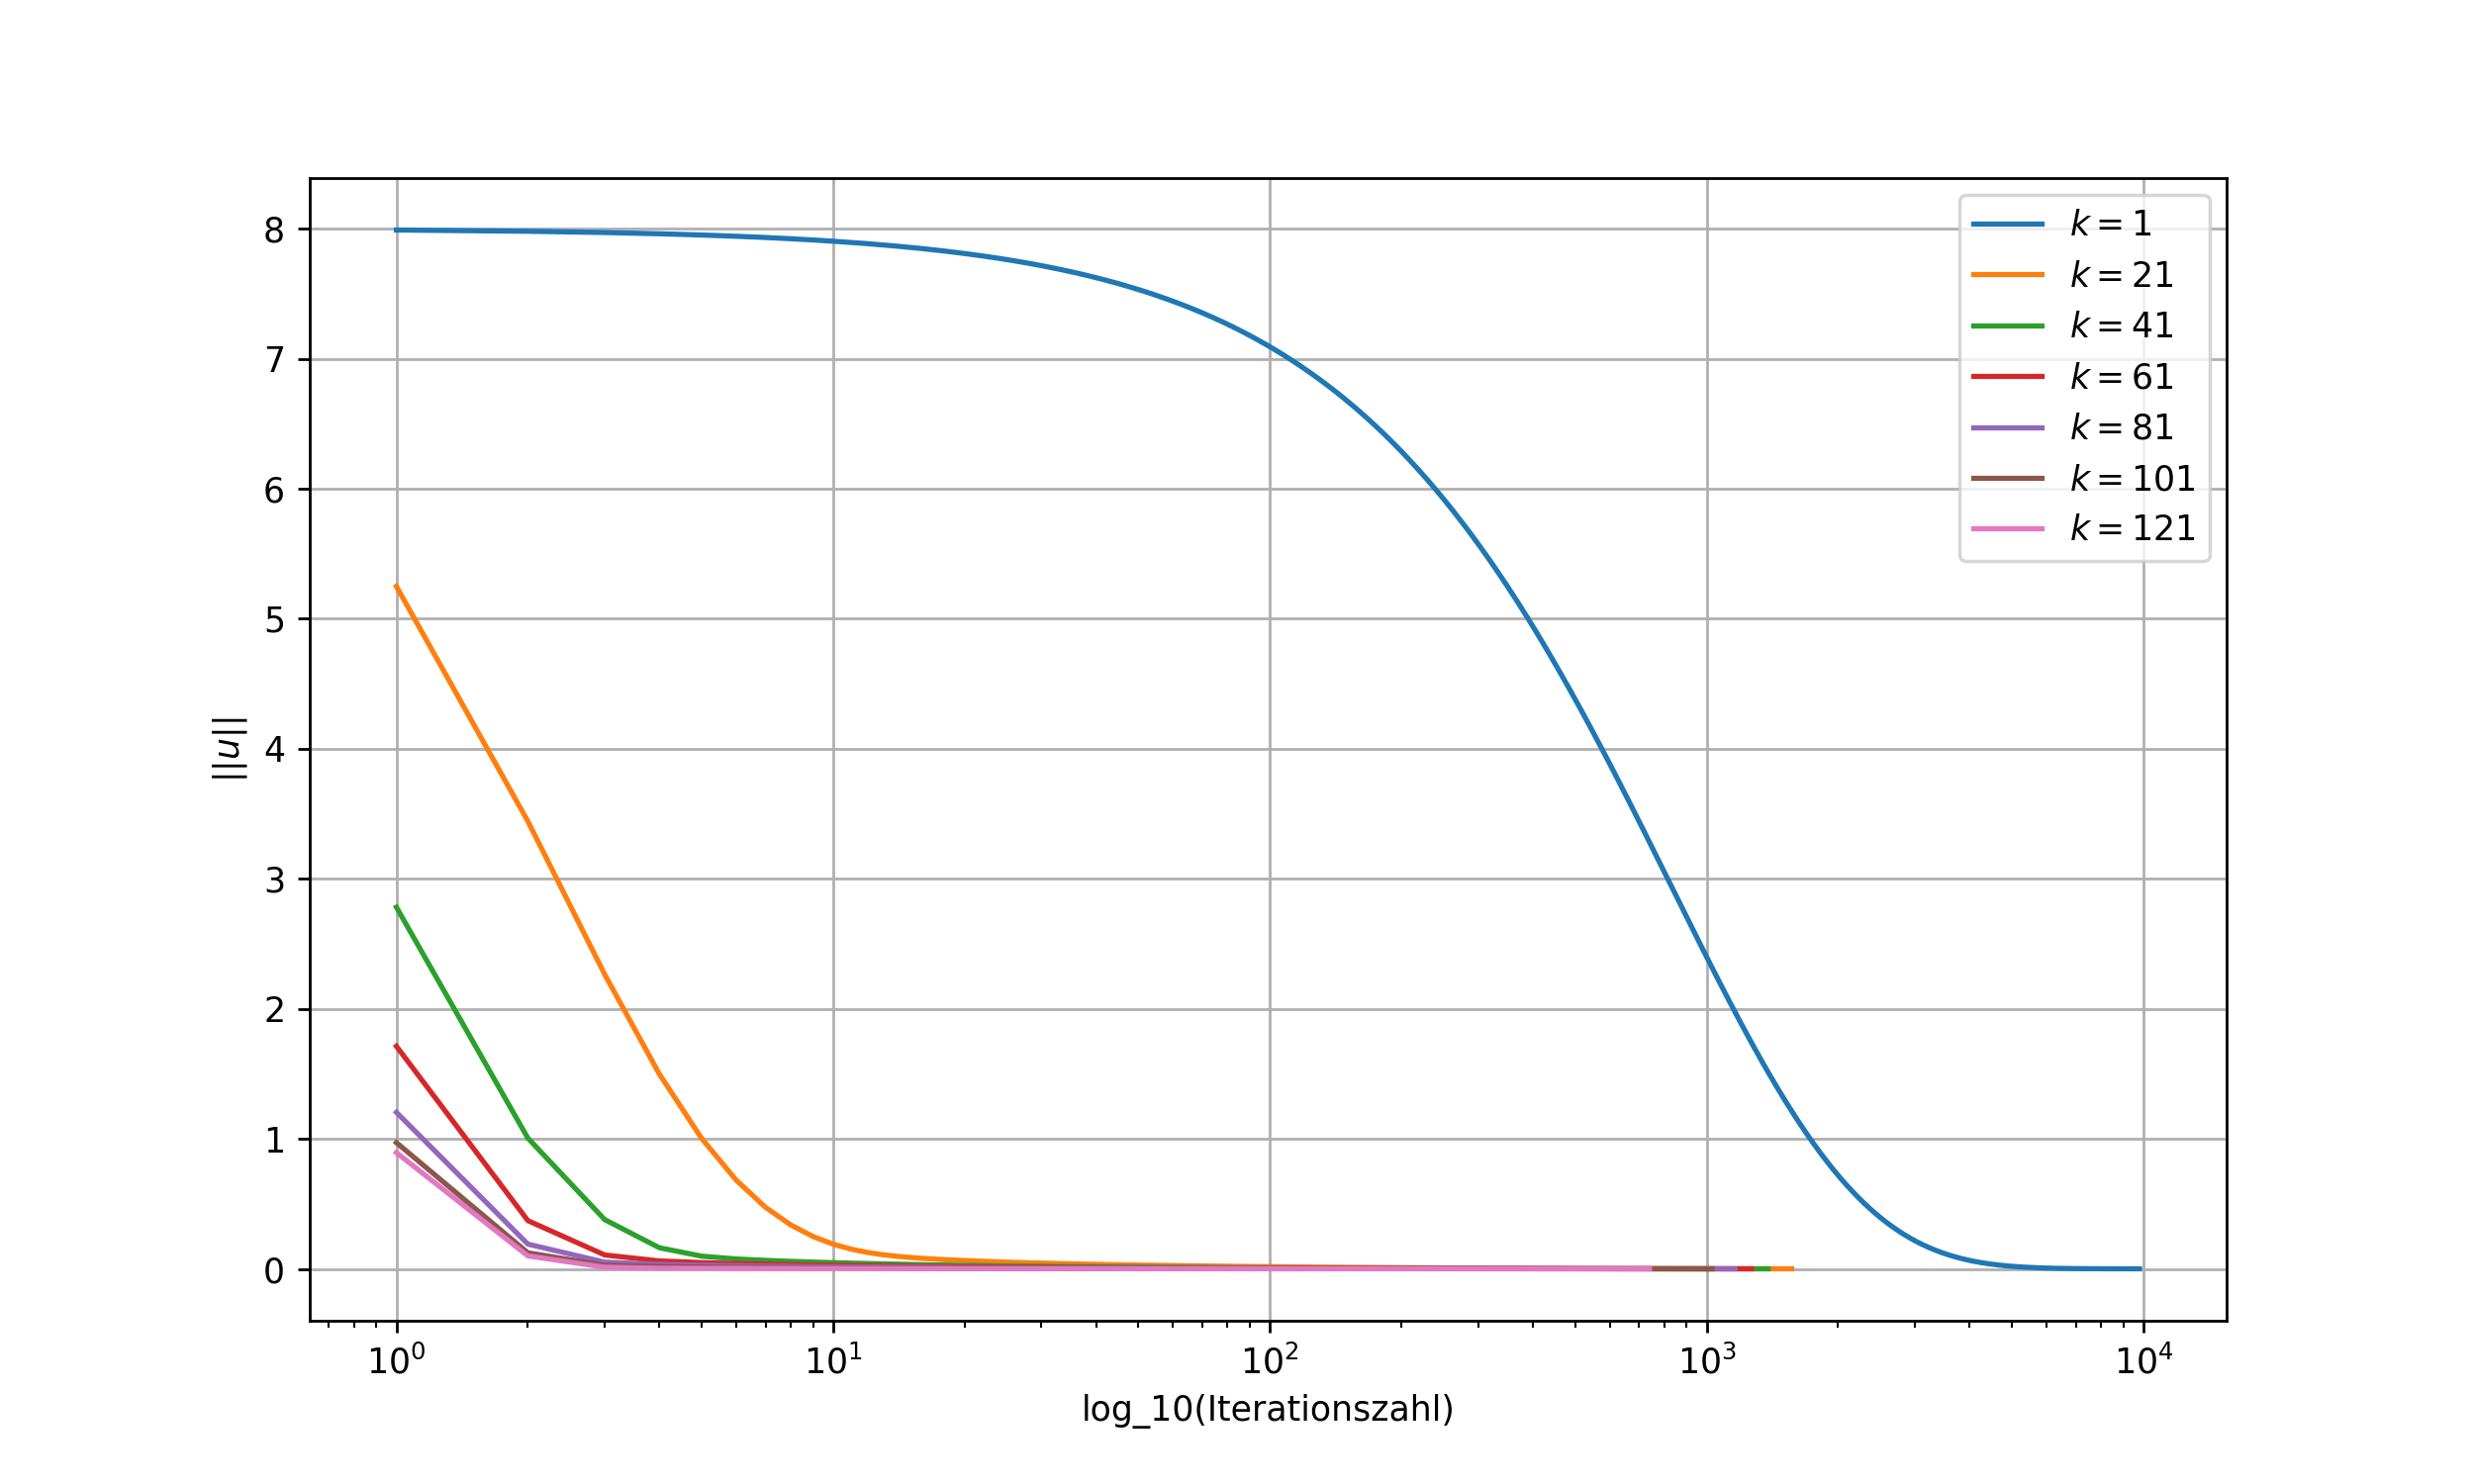
\includegraphics[width=0.6\textwidth,scale=0.7]{h1_comparison_plot_1}
    \caption[Vergleich der Dämpfungswirkung des Gauß-Seidel-Verfahrens für verschiedene Wellenzahlen.]{Vergleich der Dämpfungswirkung des Gauß-Seidel-Verfahrens für verschiedene Wellenzahlen.}\label{fig:h1_comparison_plot_1}
\end{figure} In Abbildung \ref{fig:h1_comparison_plot_1} ist zu erkennen, dass die Dämpfungswirkung des Gauß-Seidel-Verfahrens für größer werdende Wellenzahlen extrem schnell zunimmt, da dann die Norm der Näherungslösung bereits nach wenigen Iterationen sich wie die Norm der exakten Lösung verhält.\newline

\noindent 3. In diesem Aufgabenteil wird das Ziel verfolgt, die Dämpfungswirkung durch das Multigrid-Verfahren zu verifizieren. Dafür werden die Level $1$, $2$, $3$, $4$ und $5$ verwendet. Als Abbruchkriterium wird wieder die absolute Genauigkeit $\epsilon_{\mathrm{abs}} = 0.1 h^2$ verwendet.
Außerdem wird auf jedem Level $\nu_{\mathrm{pre}} = \nu_{\mathrm{post}} = 1$ als Glättungsschritt benutzt. Um die Dämpfungswirkung der verschiedenen Level zu vergleichen, wird für jedes Level die Norm der Näherungslösung gegen die Iterationszahl für die Wellenzahlen $k = 1, 41, 81, 121$ dargestellt
(siehe Abbildungen \ref{fig:h1_level1}, \ref{fig:h1_level2}, \ref{fig:h1_level3}, \ref{fig:h1_level4} und \ref{fig:h1_level5}).
\begin{figure}[htbp]
    \centering
    \begin{minipage}{0.45\linewidth}
        \centering
        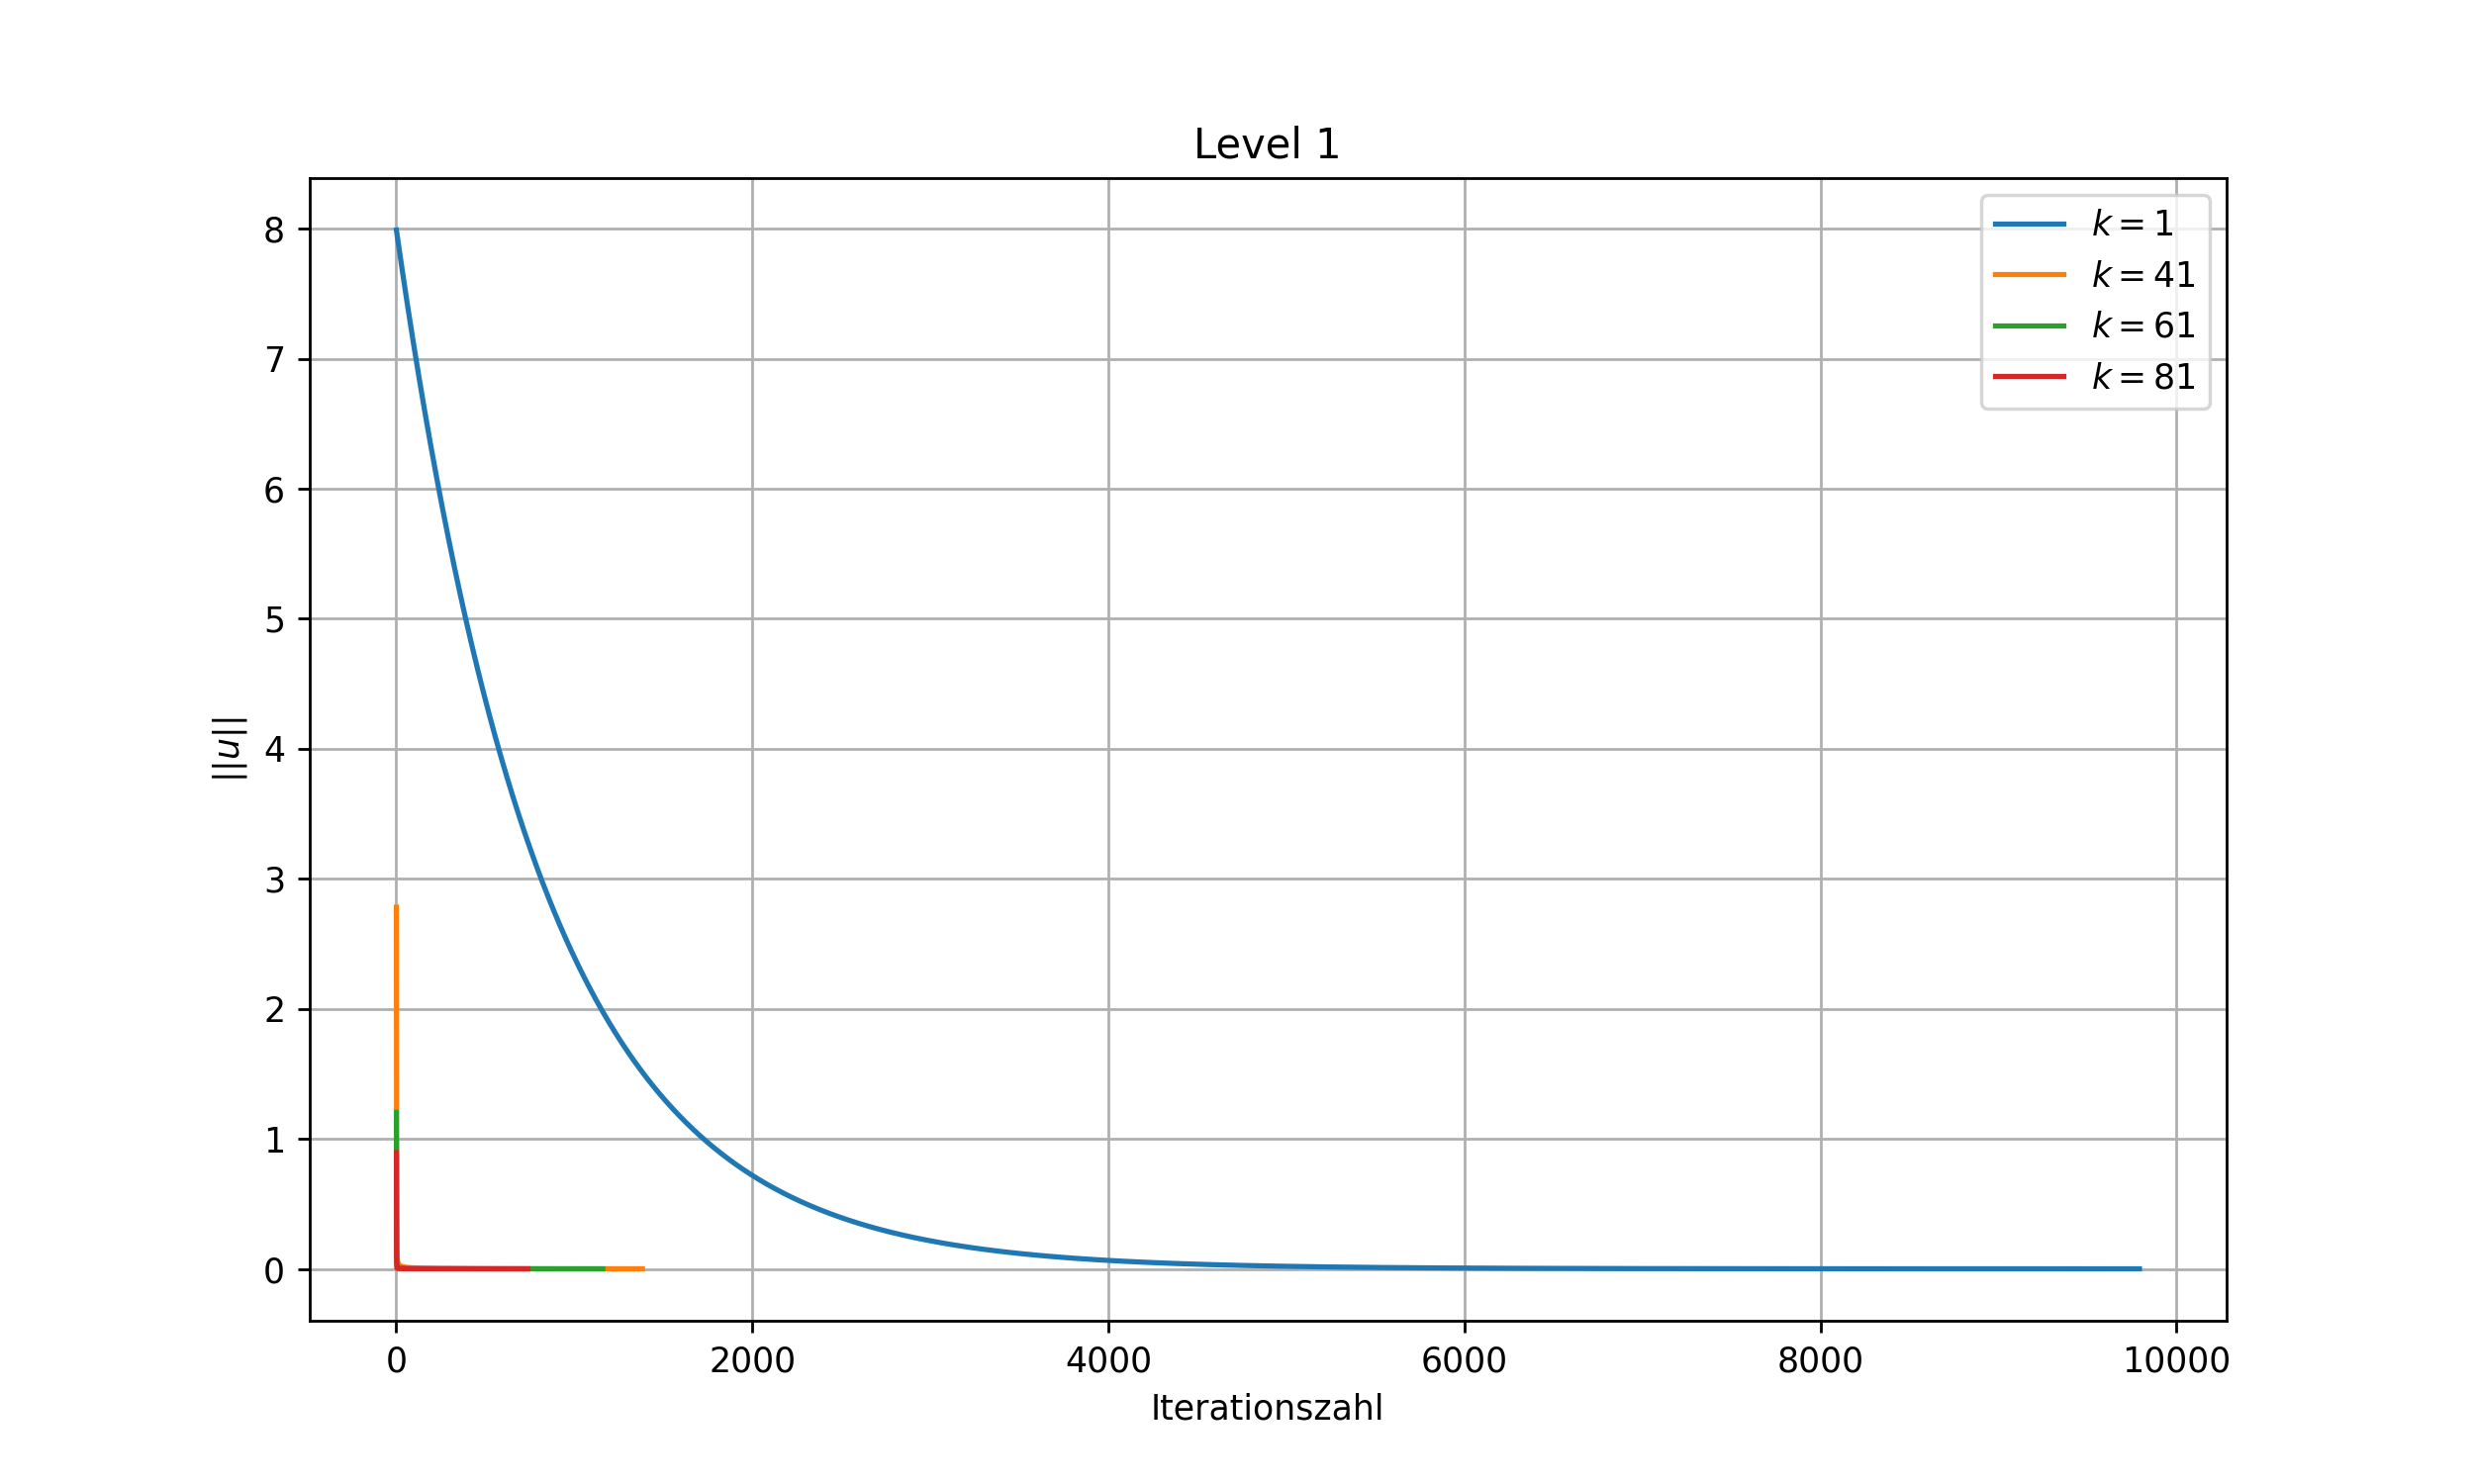
\includegraphics[width= \linewidth,scale=0.7]{h1_level1}
        \caption[Level 1]{Dämpfungswirkung Level 1}\label{fig:h1_level1}
    \end{minipage}
     \hspace{0.5cm}
    \begin{minipage}{0.45\linewidth}
        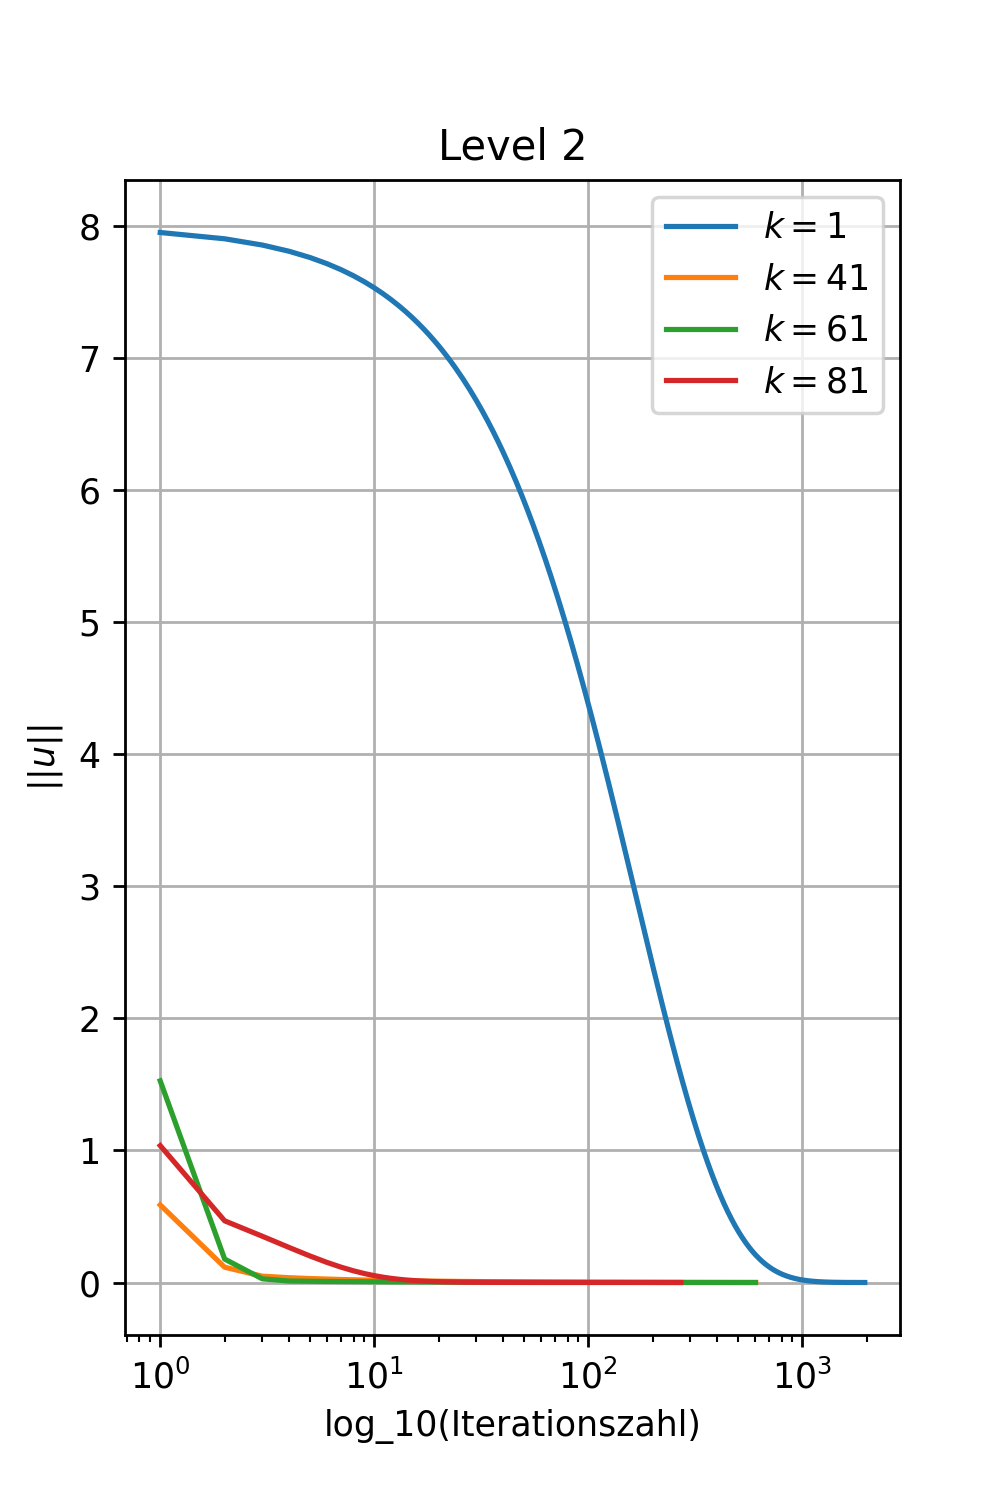
\includegraphics[width=\linewidth,scale=0.7]{h1_level2}
        \caption[Level 2]{Dämpfungswirkung level 2}\label{fig:h1_level2}
    \end{minipage}
\end{figure}
\begin{figure}[htbp]
    \centering
    \begin{minipage}{0.45\linewidth}
        \centering
        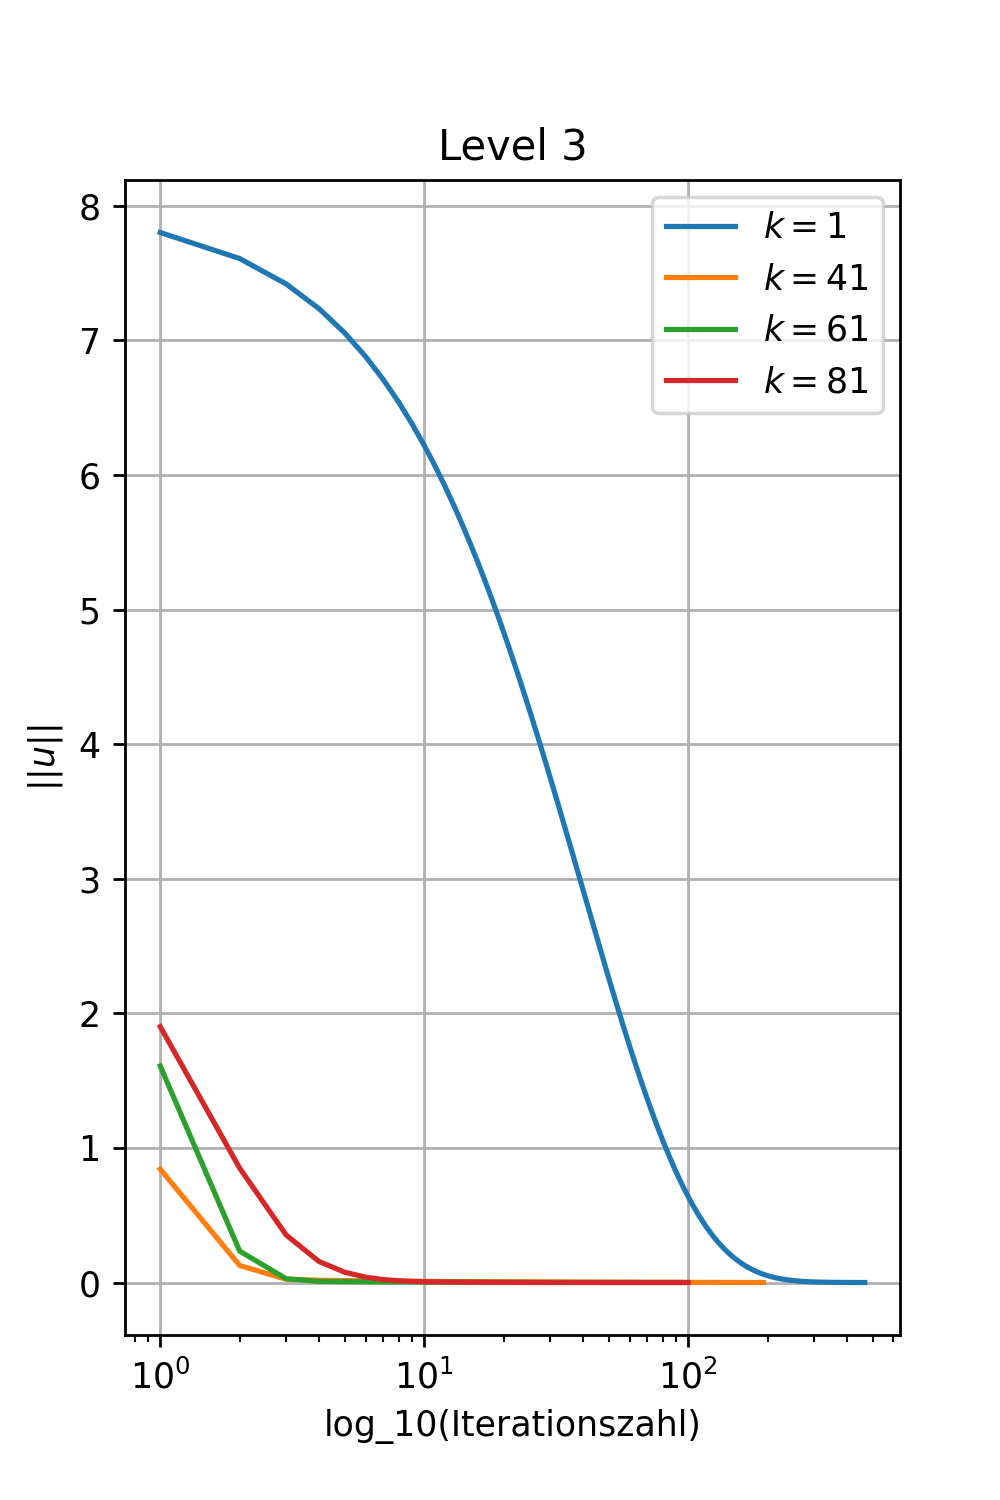
\includegraphics[width= \linewidth,scale=0.7]{h1_level3}
        \caption[Level 3]{Dämpfungswirkung Level 3}\label{fig:h1_level3}
    \end{minipage}
     \hspace{0.5cm}
    \begin{minipage}{0.45\linewidth}
        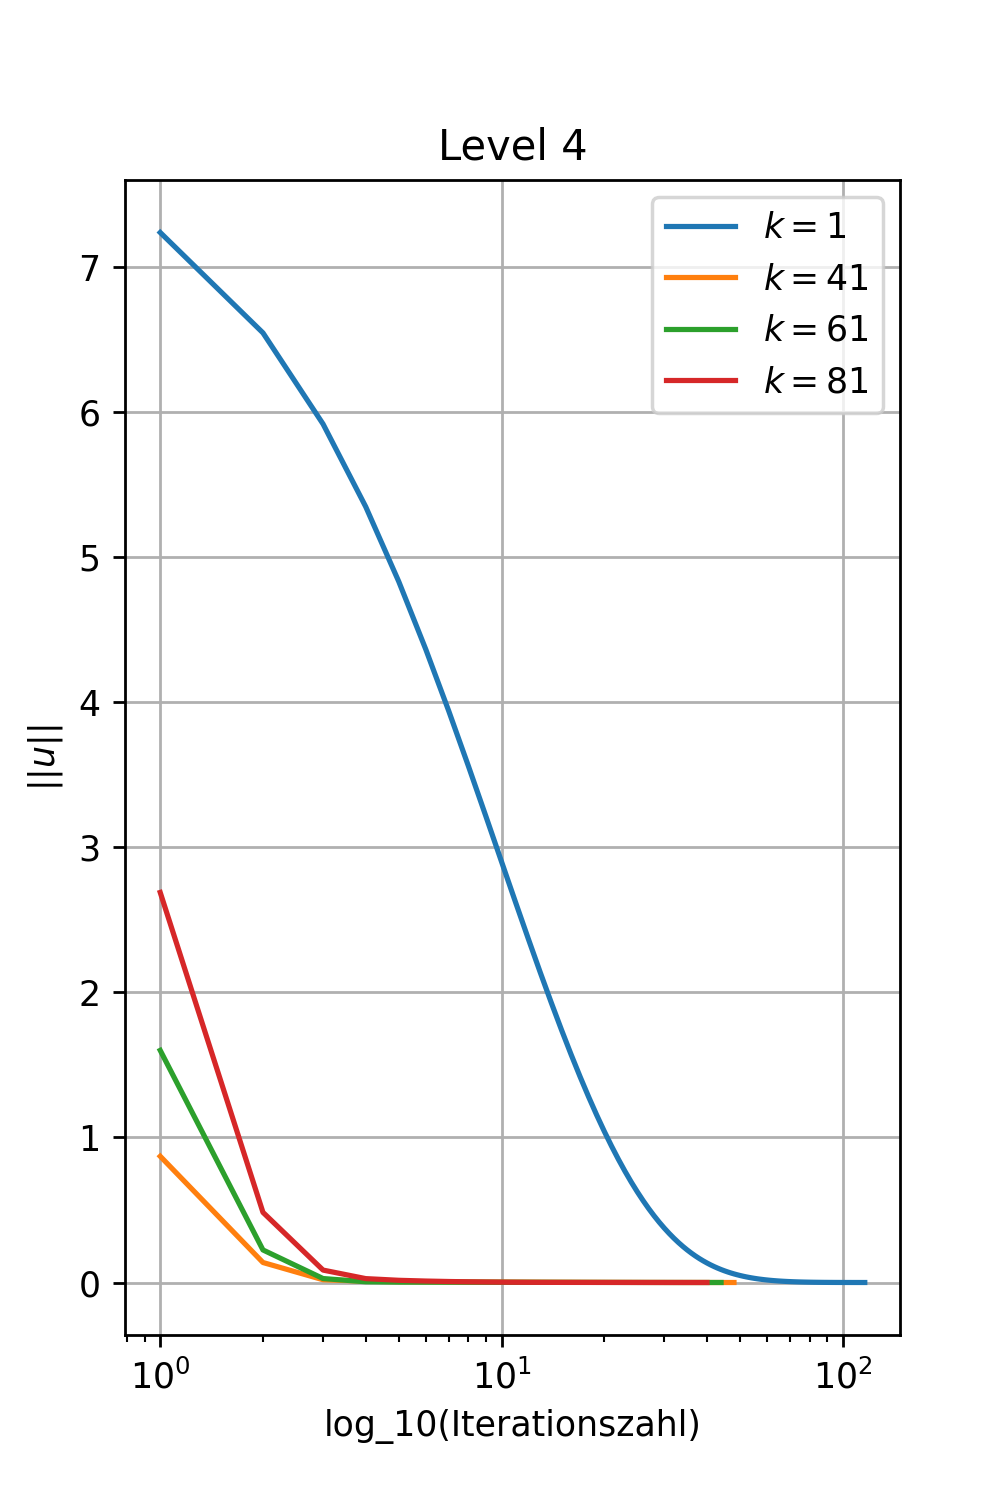
\includegraphics[width=\linewidth,scale=0.7]{h1_level4}
        \caption[Level 4]{Dämpfungswirkung level 4}\label{fig:h1_level4}
    \end{minipage}
\end{figure}
\begin{figure}[htbp]
    \centering
    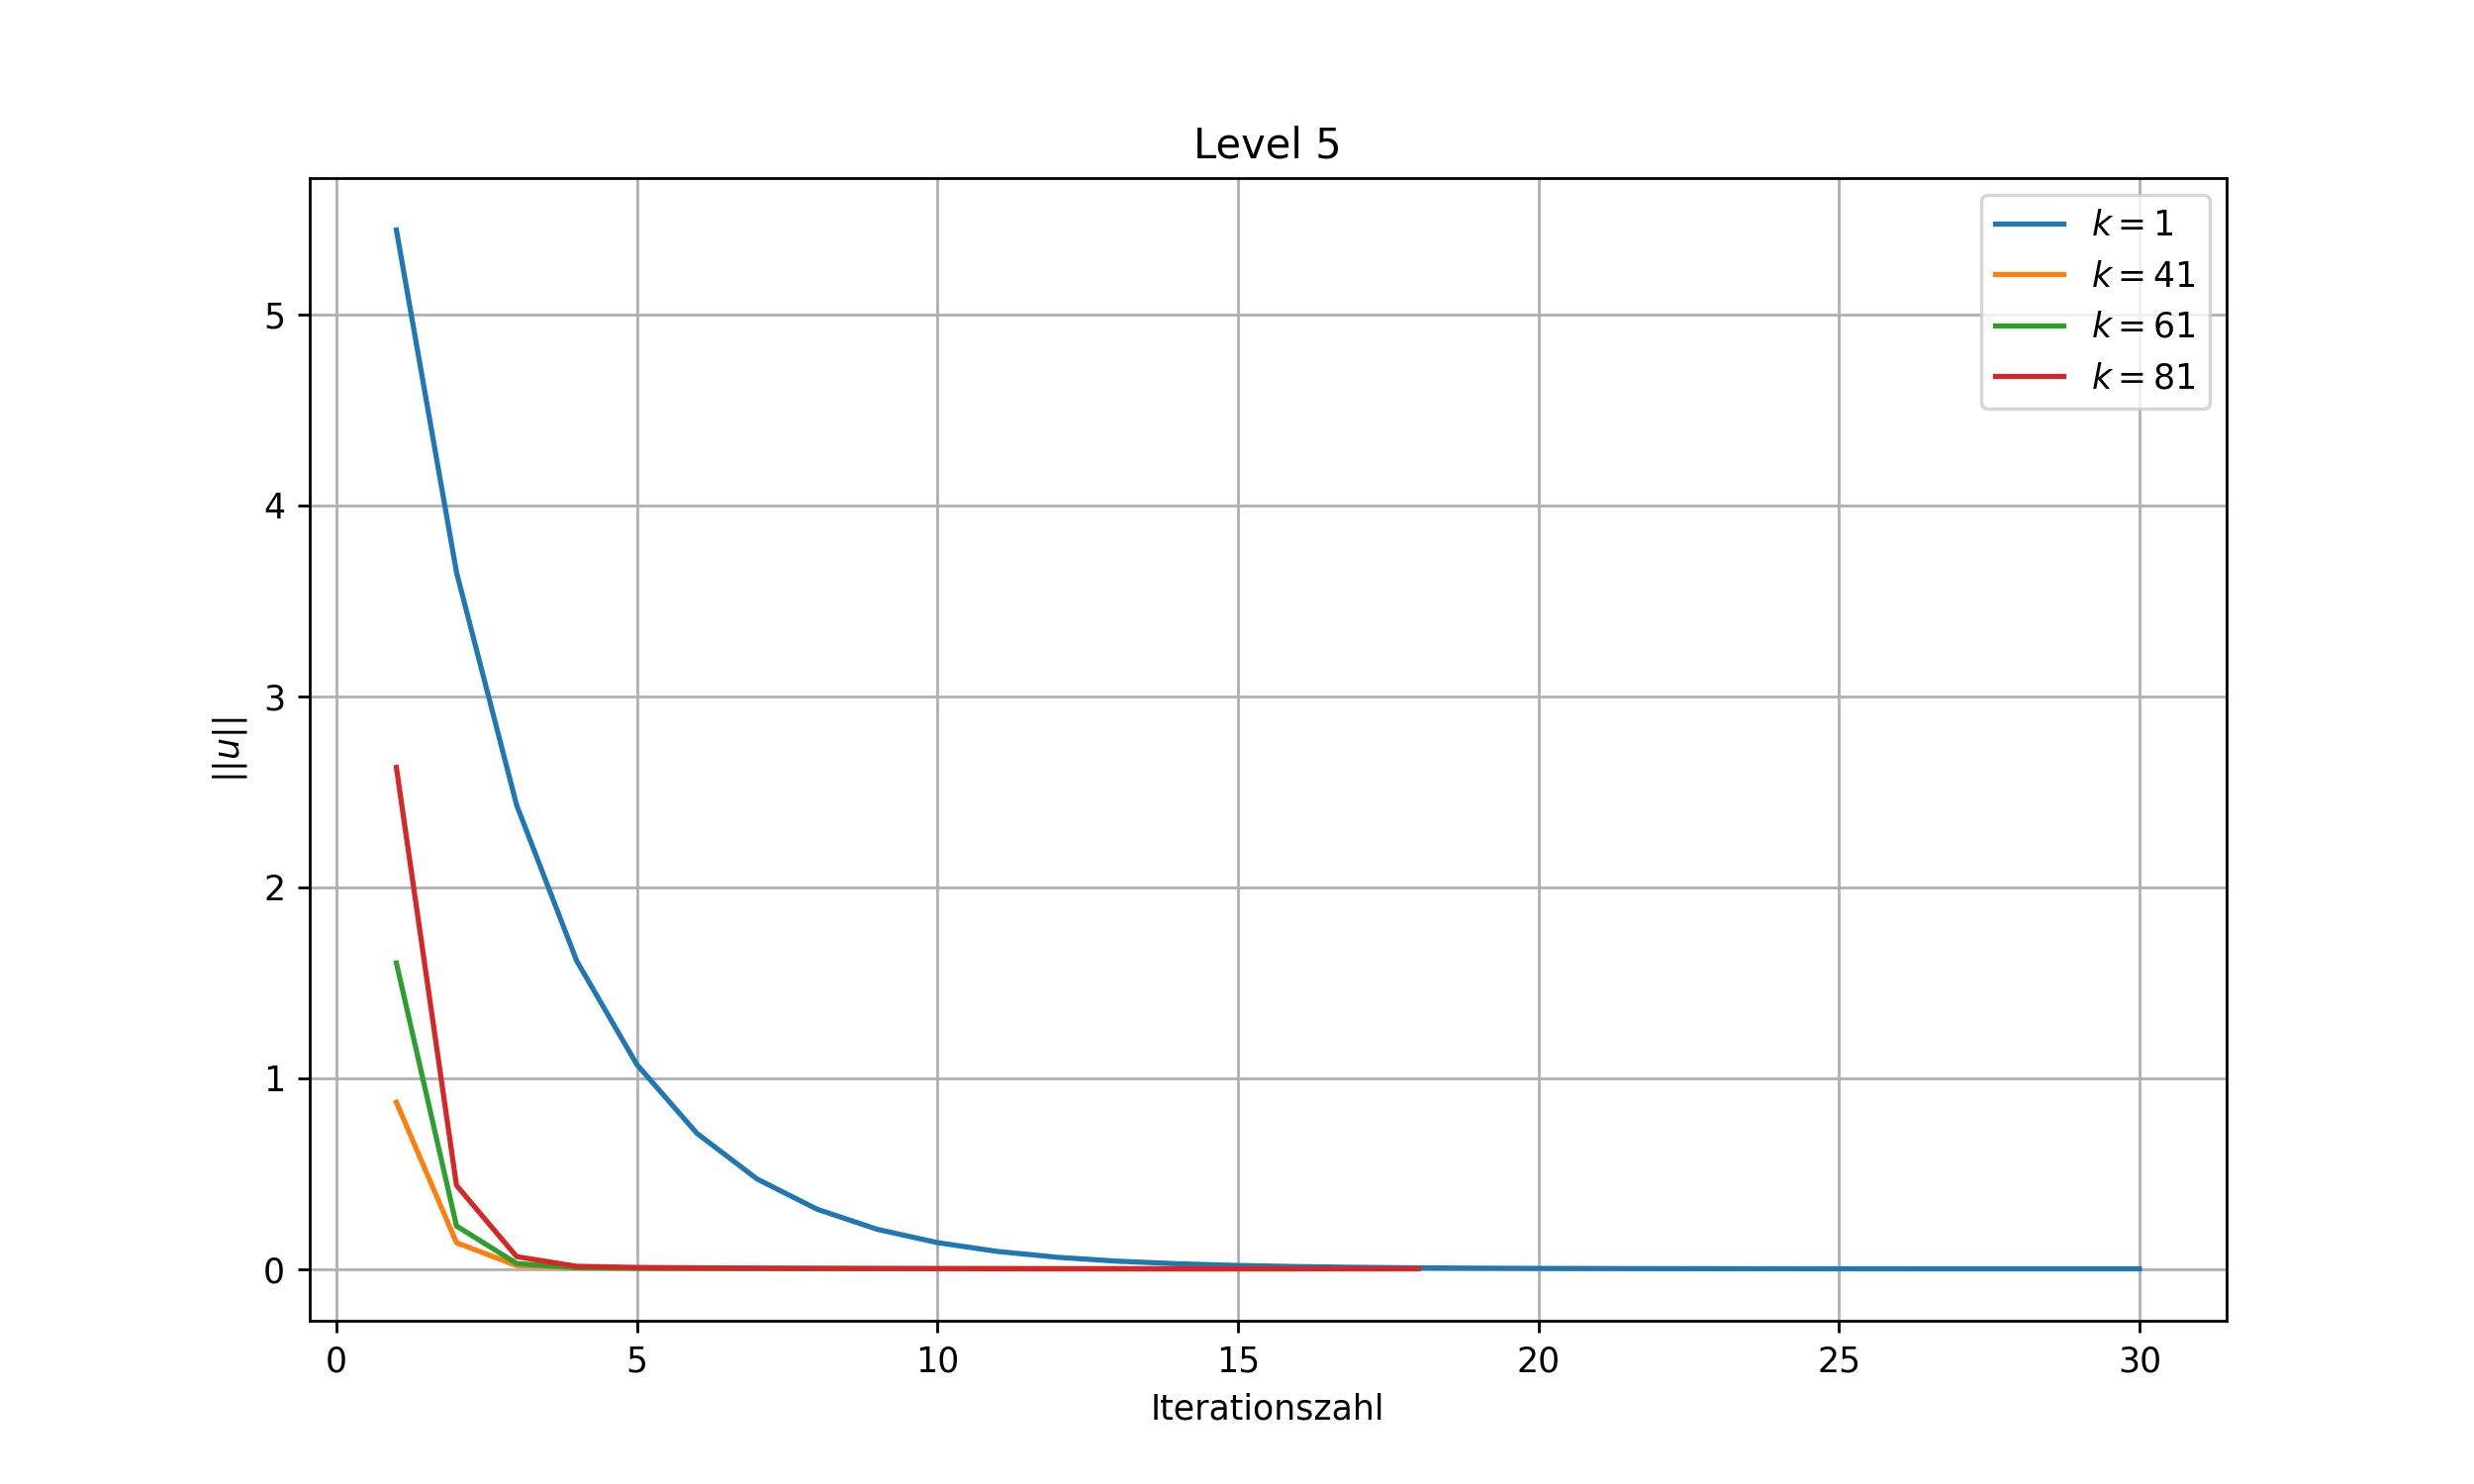
\includegraphics[width=0.5\linewidth]{h1_level5}
    \caption[Dämpfungswirkung des Multigrid-Verfahrens bei Level 5.]{Dämpfungswirkung des Multigrid-Verfahrens bei Level 5.}\label{fig:h1_level5}
\end{figure} Tatsächlich ist eine Steigerung der Dämpfungswirkung durch das Multigrid-Verfahren zu erkennen, da bei steigendem Level des Multigrid-Verfahrens für verschiedene Wellenzahlen immer weniger Iterationsschritte benötigt werden, sodass die Norm der Näherungslösung
gegen die Norm der exakten Lösung konvergiert. Um diese Verbesserung eindeutig zu erkennen, werden nochmal die verschiedenen Level in einem gemeinsamen Plot dargestellt (siehe Abbildung \ref{fig:h1_level_comparison}), indem für jedes Level die Norm der Näherungslösung gegen die Iterationszahl für $k = 1$ aufgetragen wird.
\begin{figure}[htbp]
    \centering
    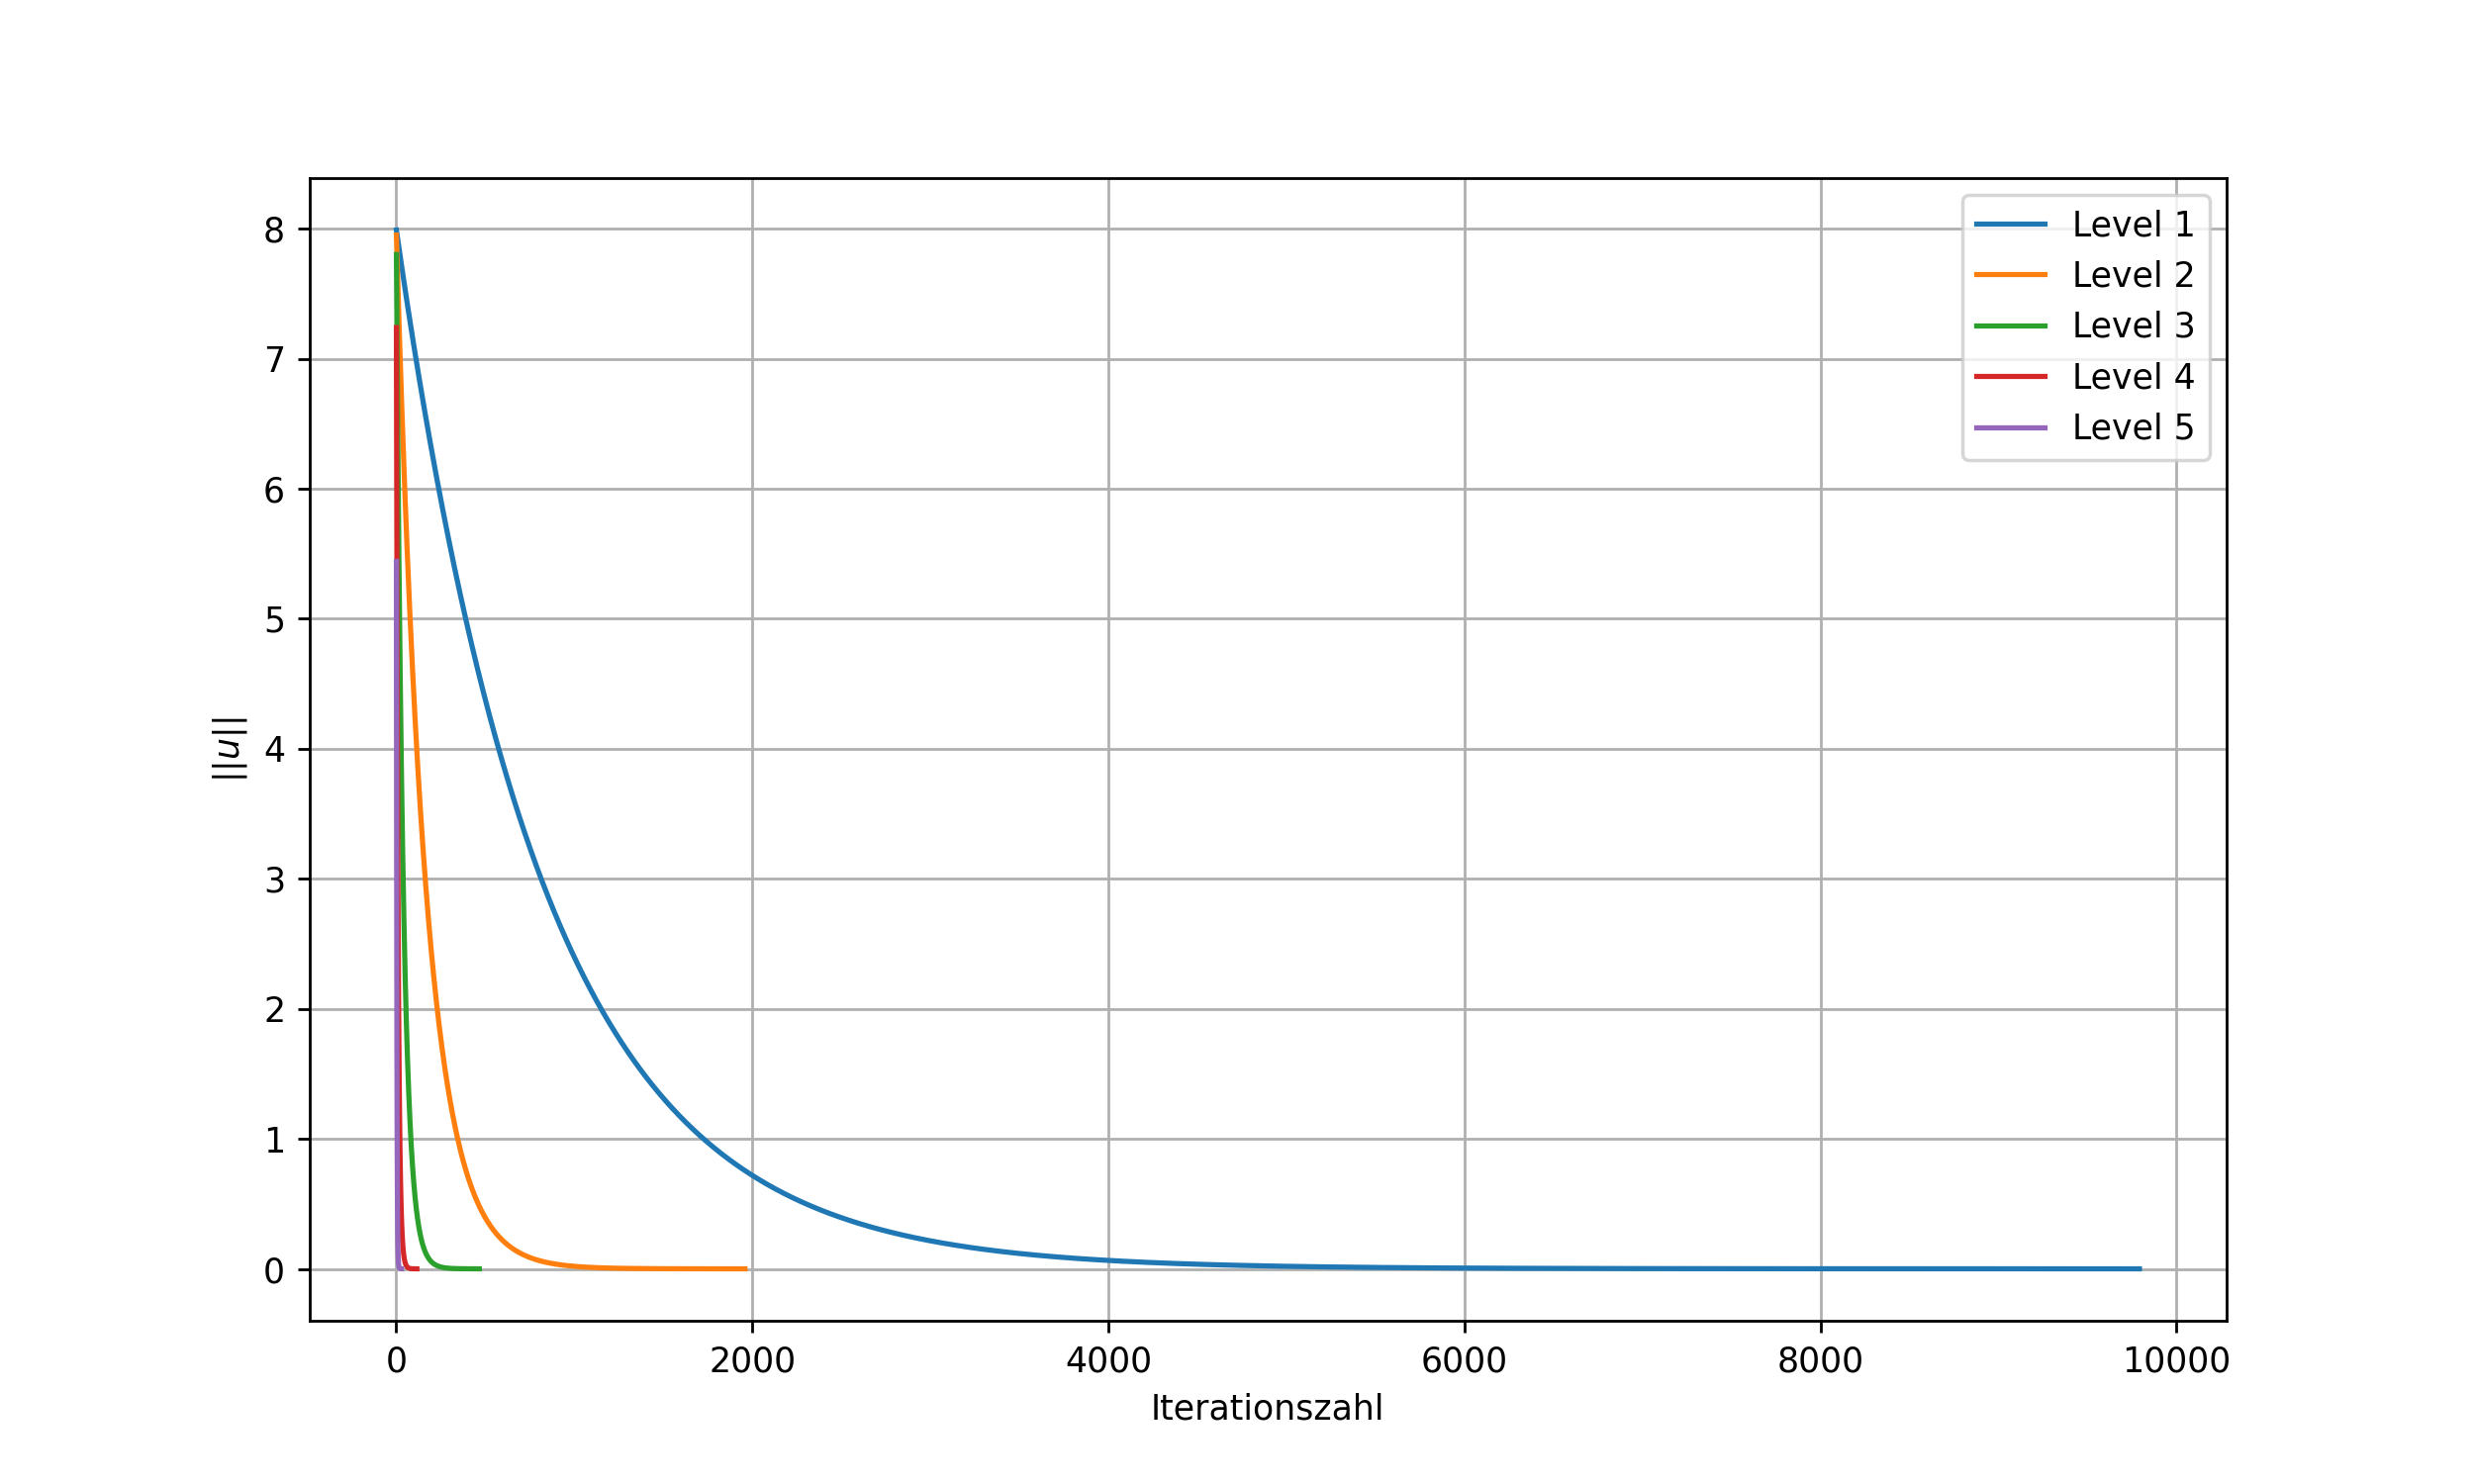
\includegraphics[width=0.6\textwidth,scale=0.7]{h1_level_comparison}
    \caption[Verbesserung der Dämpfungswirkung durch das Multigrid-Verfahren.]{Verbesserung der Dämpfungswirkung durch das Multigrid-Verfahren.}\label{fig:h1_level_comparison}
\end{figure} Somit lässt sich als Ergebnis festhalten, dass sich mit dem Multigrid-Verfahren die Dämpfungswirkung verbessern lässt, womit numerische Lösungen von Differentialgleichungen letztlich durch wenige Iterationen schnell und effizient bestimmt werden können.\newpage

\section*{H.2: Diskretisierungsunabhängige Konvergenzgeschwindigkeit}\label{sec:h2}

In dieser Aufgabe wird das folgende Randwertproblem betrachtet:
\begin{equation*}
    u''(x) - \omega^2 u(x) = s(x) = -\frac{1}{2} x \mathrm{e}^{-x} , \quad u(0) = 0 , \quad \lim_{x \to \infty} u(x) = 0.
\end{equation*} Hierbei wird die Randbedingung bei großen $x$ durch $u(x) = 0$ für $x \geq R_{\mathrm{max}} = 20$ approximiert. Außerdem wird $\omega = 1$ gesetzt.\\ \\
1. Zuerst soll eine Erwartung an den Effizienzgewinn durch Einsatz des Multigrid-Verfahrens für das gegebene Randwertproblem gegeben werden. Aus der Vorlesung ist bekannt, dass für das Multigrid-Verfahren eine gute Glättung erwartet wird, wenn die Amplitude
der Fourier-Transformierten von $s(t) = -\frac{1}{2}t \mathrm{e}{-t}$ \\

\noindent 2. Für diesen Aufgabenteil (und die weiteren Aufgabenteile) wird das Multigrid-Verfahren mit V-Zyklus für das gegebene Randwertproblem mit Diskretisierung $x_j = j \cdot h$, $j = 0 , \dots 2^N$ implementiert, wobei analog
wie in der ersten Aufgabe vorgegangen wird. Hierbei soll $2^N = 8$ immer das gröbste Gitter darstellen. Auf diesem Gitter wird dann das entstehende lineare Gleichungssystem mit dem in der Vorlesung vorgestellten Tridiagonalmatrix-Algorithmus gelöst.
In jedem Fall wird $\nu_{\mathrm{pre}} = \nu_{\mathrm{post}} = 1$ und Relaxationsparameter $R = 1$ für das Gauß-Seidel-Verfahren verwendet. \\

\noindent 3. Zunächst wird die Konvergenzgeschwindigkeit mit dem Multigrid-Verfahren mit nur einem Level (Gauß-Seidel-Verfahren) für feinste Gitter mit $N = 4,6,8,10,12$ verglichen, indem die Norm des Residuums in Abhängigkeit von der
Iterationszahl dargestellt wird. Bei der Implementierung wird die relative Genauigkeit $\epsilon_{\mathrm{rel}} = 10^{-3} \cdot h^2$ (relativ zur Norm von $s(x)$) verwendet.
\begin{figure}[h]
    \centering
    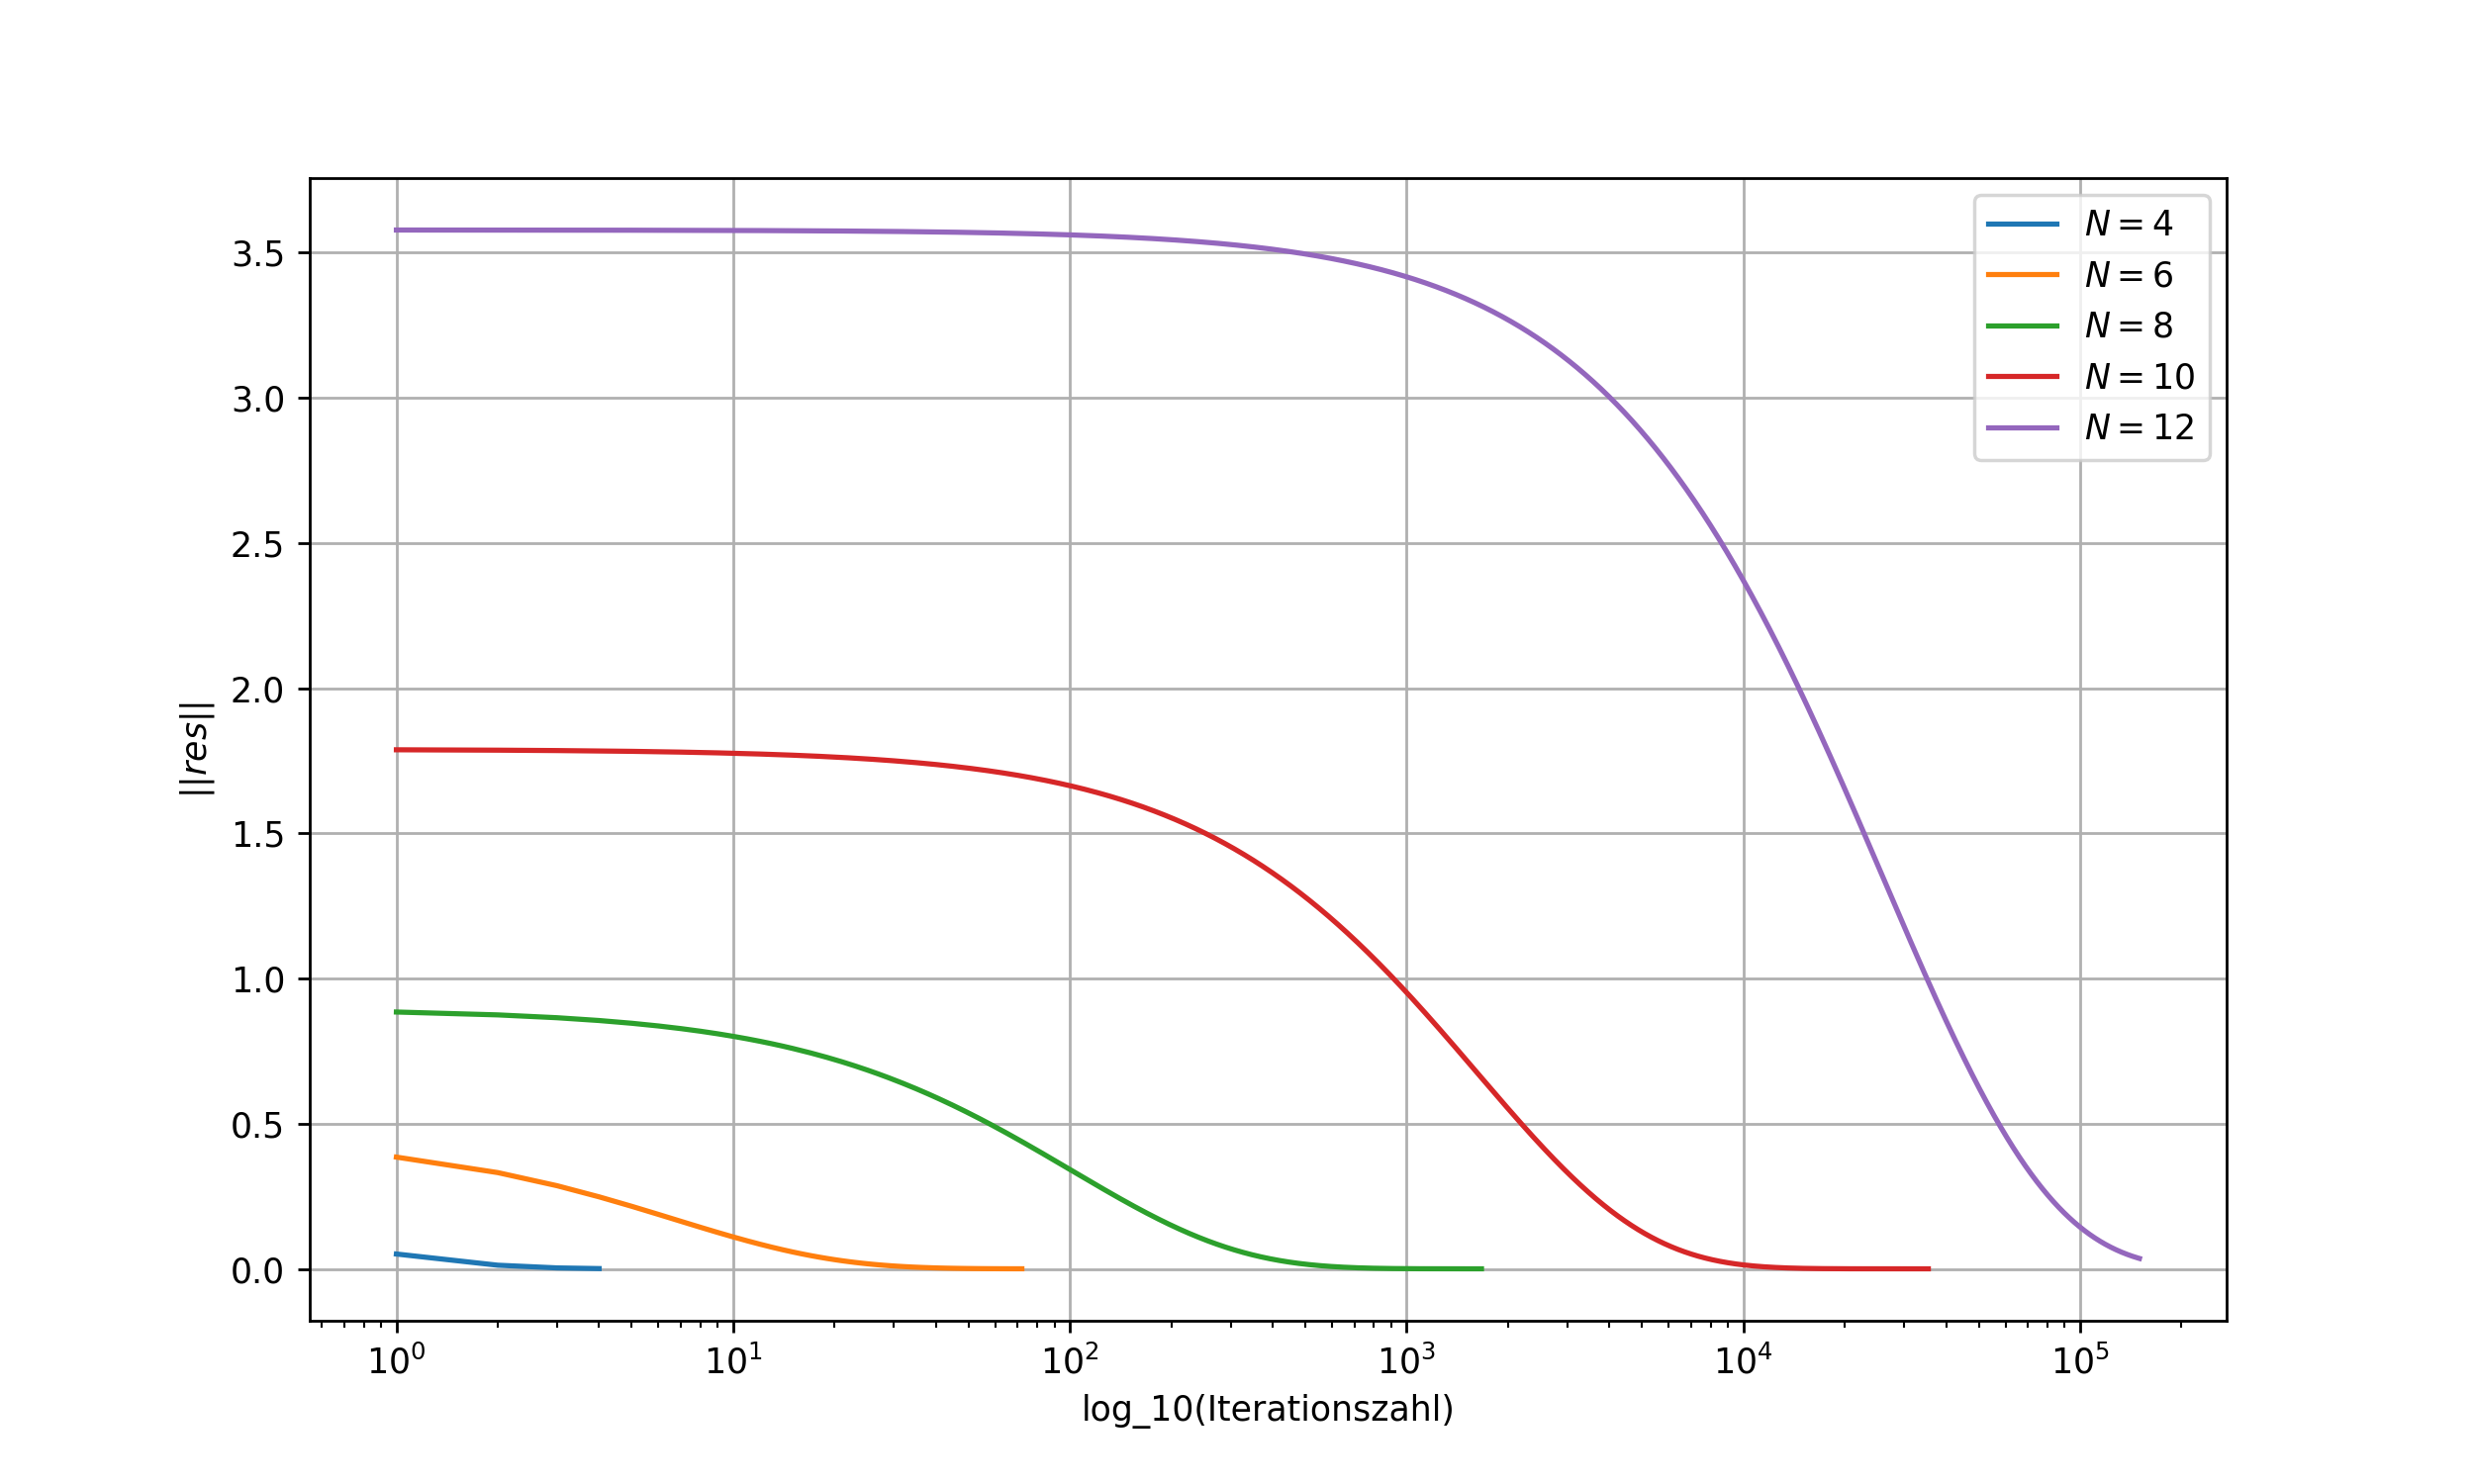
\includegraphics[width=0.6\textwidth]{h2_N_comparison_1}
    \caption[Vergleich der Konvergenzgeschwindigkeit des Gauß-Seidel-Verfahrens für $N = 4,6,8,10,12$.]{Vergleich der Konvergenzgeschwindigkeit des Gauß-Seidel-Verfahrens für $N = 4,6,8,10,12$.}\label{fig:h2_N_comparison_1}
\end{figure} In der Abbildung \ref{fig:h2_N_comparison_1} ist der Vergleich der Konvergenzgeschwindigkeit für verschiedene $N$ dargestellt. Es ist zu erkennen, dass
die Konvergenzgeschwindigkeit für kleinere $N$ stark zunimmt, da weniger Iterationen benötigt werden, sodass die Norm des Residuums gegen $0$ konvergiert.\\

\noindent 4. In diesem Aufgabenteil wird geprüft, wie die Konvergenzgeschwindigkeit mit dem Multigrid-Verfahren von der Schrittweite $h$ abhängt. Dafür wie die für jedes gewählte $N$ die Anzahl
der zur Konvergenz benötigten Iterationen verglichen. Auch hier wird wieder die relative Genauigkeit $\epsilon_{\mathrm{rel}} = 10^{-3} \cdot h^2$ als Abbruchkriterium verwendet. Die Ergebnisse sind in der Abbildung
\ref{fig:h2_last_plot} dargestellt.
\begin{figure}[ht]
    \centering
    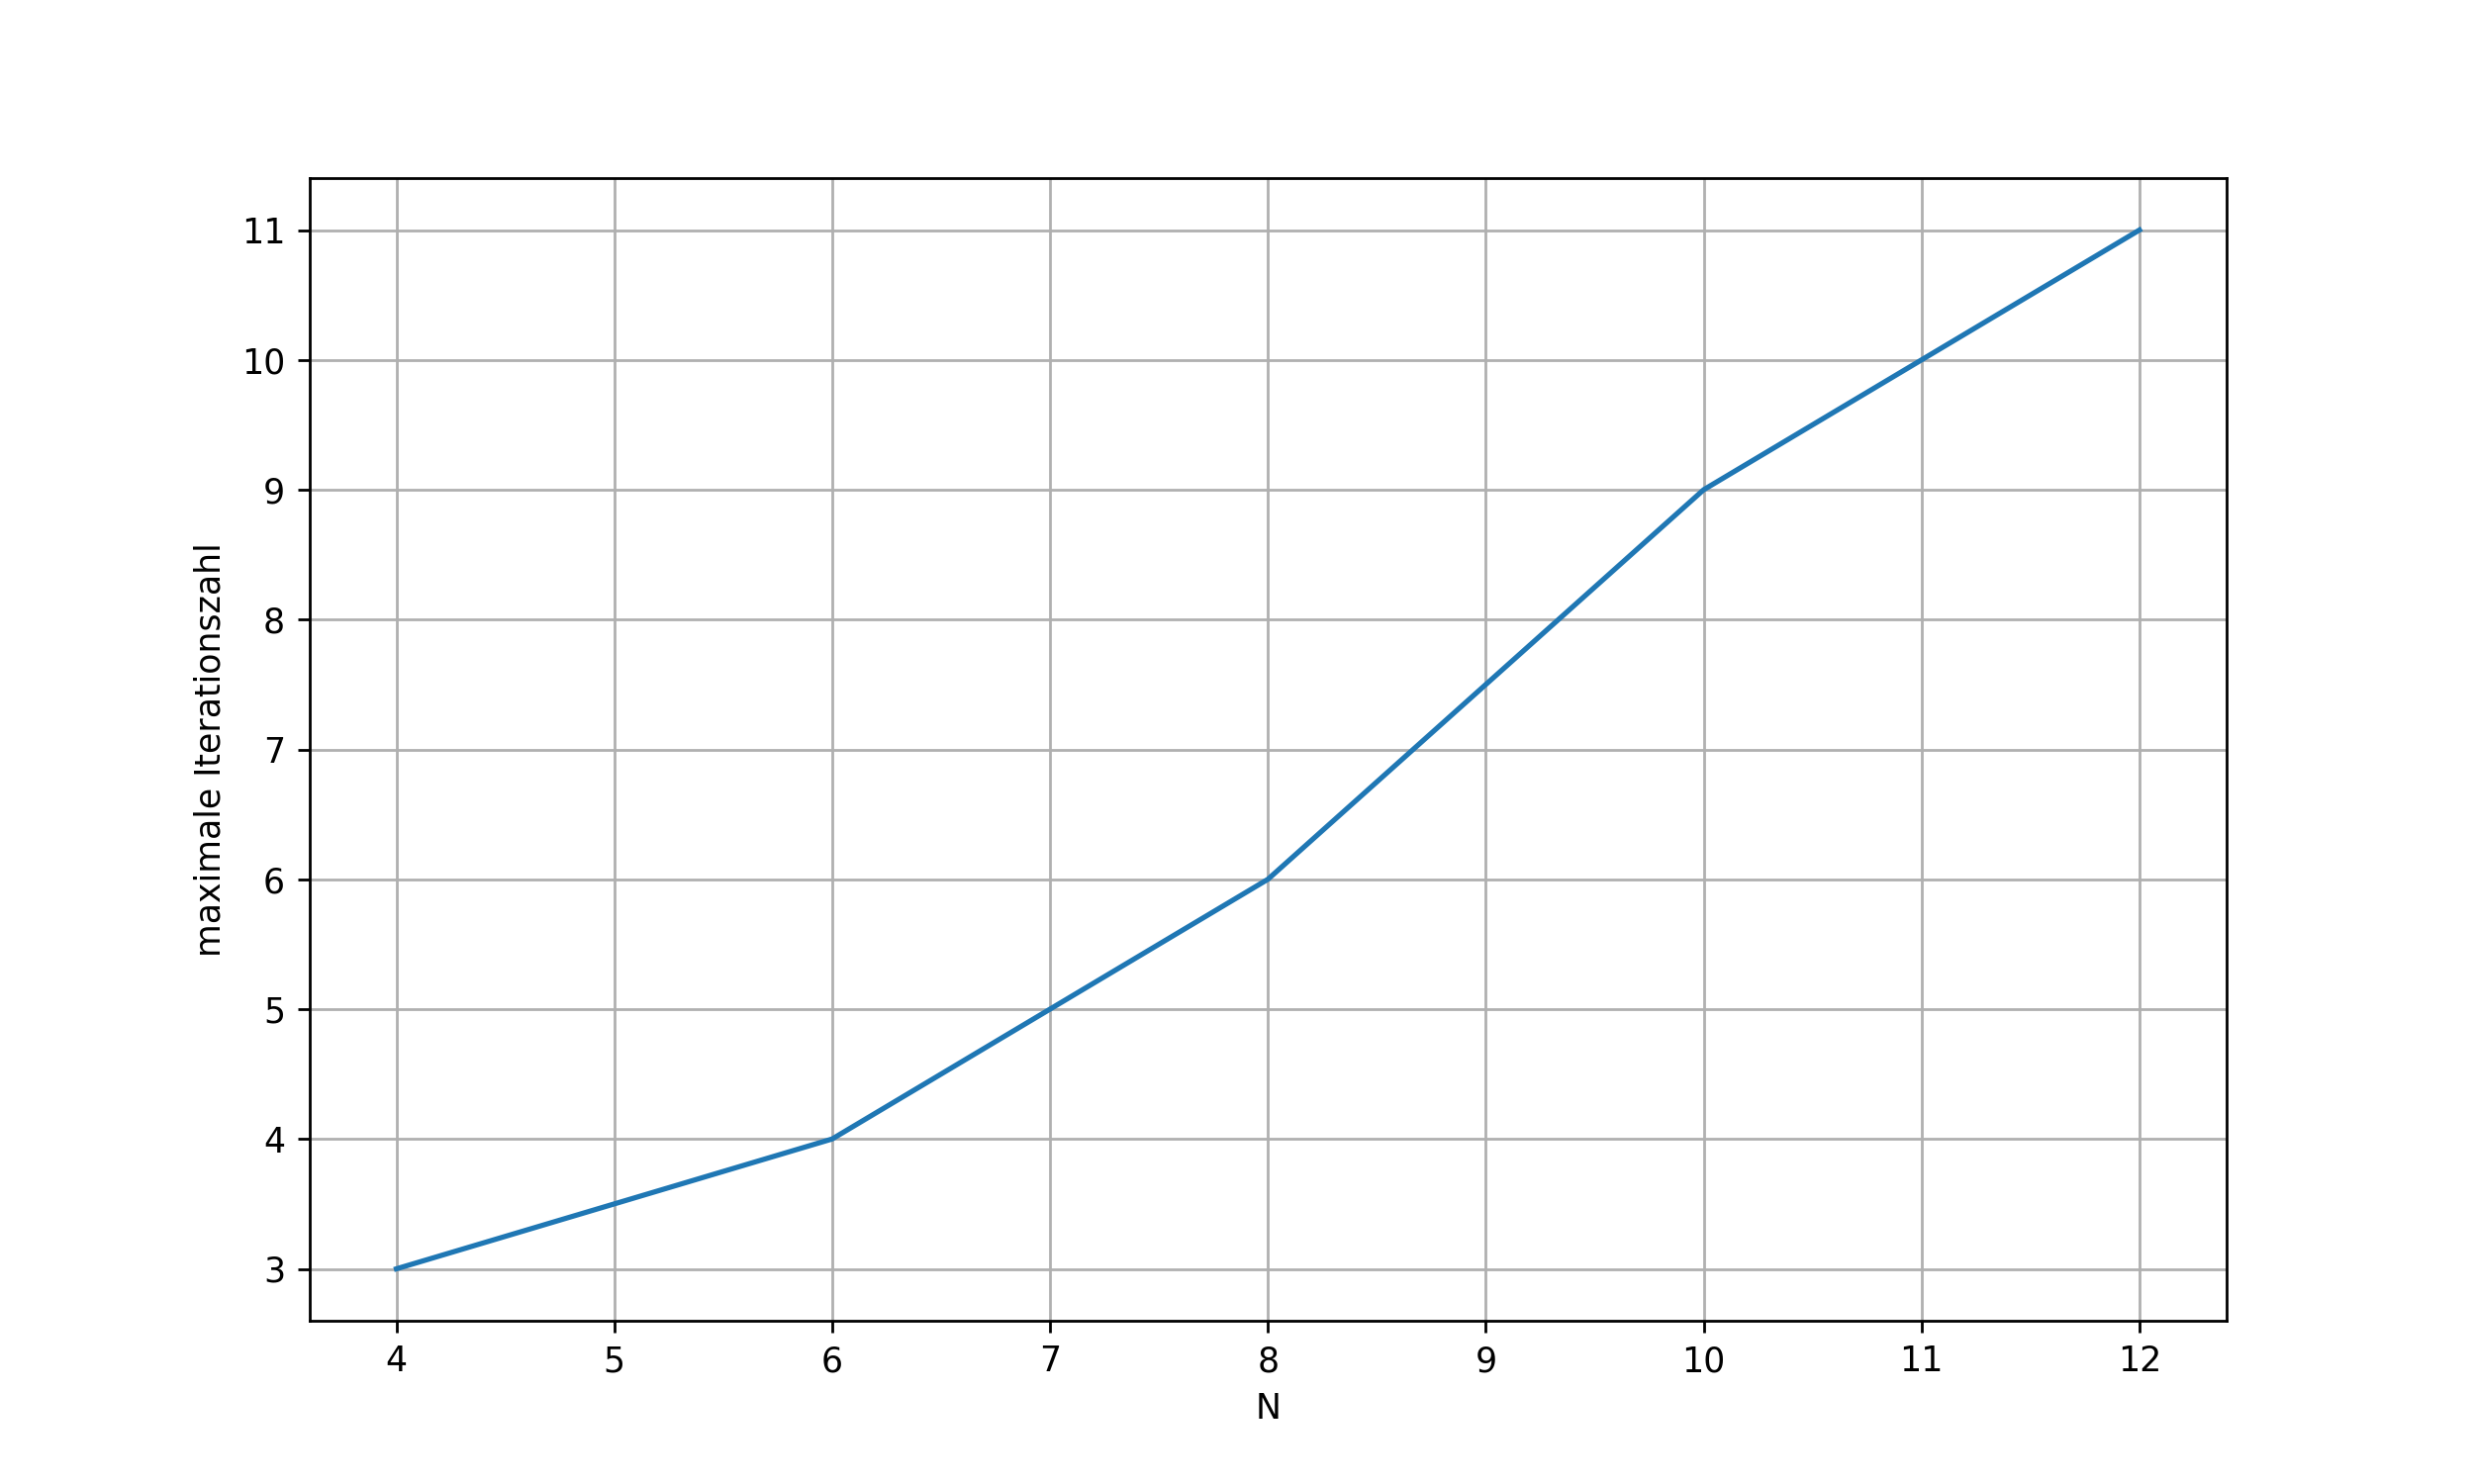
\includegraphics[width=0.6\textwidth]{h2_last_plot}
    \caption[Vergleich der Konvergenzgeschwindigkeit.]{Vergleich der Konvergenzgeschwindigkeit.}\label{fig:h2_last_plot}
\end{figure} Es ist zu erkennen, dass bei verschiedenen Werten $N$ die Konvergenzgeschwindigkeit für höhere Level des Multigrid-Verfahrens extrem stark zunimmt. \\
Somit kann als Ergebnis festgehalten werden,
 dass die Konvergenzgeschwindigkeit des Multigrid-Verfahrens für größer werdende Level zunimmt, was gröber werdenden Gittern und einer größer werdenden Schrittweite entspricht.\\
Dies ist nicht das zu erwartende Ergebnis, da eine von der Schrittweite unabhängige Konvergenzgeschwindigkeit erwartet wurde.

\newpage

\listoffigures

\end{document}